\documentclass[a4paper, 20pt]{article}
\usepackage{graphicx}
\usepackage{amsmath}
\usepackage[a4paper, total={6in, 8in}]{geometry}
\geometry{top=1mm,textheight=260mm}
\title{\textbf{ EE301A : Digital Signal Processing }\\ Computer Assignment I}
\author{Ankush Singh 150107}
\begin{document}
\maketitle
\hline\hline
\vspace{0.4pc}
Ans 1.(a) Observe that the final output is given by :
\begin{align*}
d_n&=(b_n+jc_n)e^{-j\Theta_n} \\
\implies d_n &= b_ne^{-j\Theta_n}+c_ne^{j({\frac{\pi}{2}-\Theta_n})}\\
\end{align*}
\vspace{-1pc}
Equating the real and imaginary parts of both sides and using the relation $d_n=a_n$ we get:
\begin{align}
0=-b_n\sin(\Theta_n)+c_n\cos(\Theta_n)\\
a_n=b_n\cos(\Theta_n)+c_n\sin(\Theta_n)
\end{align}\\
Multiplying with $\cos(\Theta_n)$ in (1) and $\sin(\Theta_n)$ in (2) and adding we get:
\begin{equation}
c_n=a_n\sin(\Theta_n)
\end{equation}\\
Again multiplying with $\sin(\Theta_n)$ in (1) and with $\cos(\Theta_n)$ in (2) ,and subtracting (1) from (2) we get:
\begin{equation}
b_n=a_n\cos(\Theta_n)
\end{equation}
But it is given that $b_n =a_n\cos(\frac{n\pi}{2})$. Thus from (4) we get
 \[
 \boxed{\Theta_n = \frac{n\pi}{2}}
 \]\\
 Given $a_n=p((n-n_o)T_s)$, we observe that $a_n$ is symmetric about $n$ =50 where $ n \in \{1,2,..,100\}$.\\
 From (2) , both sides should be symmetric about n=50.\\ Since $b_n$ and $\cos(\Theta_n)$ is already symmetric about $n$ =50 , we have $b_n\cos(\Theta_n)$ symmetric about n=50.
 \vspace{2pc}
Thus $c_n\sin(\Theta_n)$ should also be symmetric about n=50.\\
We have $c_n=\hat{b_{n+n_1}}$ which is just a $n_1$ point left shifted version of $\hat{b_{n}}$.\\
$\hat{b_{n}}=b_n{\star}h_n$.
\\
From the plot of $c_n$(unshifted), we observe that it is symmetric about n=150 where $ n \in \{1,2,..,300\}$. $c_n\sin(\frac{n\pi}{2})$  is also symmetric about n=150. \\Since in order to make $d_n=a_n$, we must have $c_n\sin(\Theta_n)$ symmetric about $n$=50, we need to left the shift $c_n$ by $n$=100 so that finally it is symmetric about $n$=50. Thus , $n_1$ should be 100.
 \[
 \boxed{n_1=100}
 \]
\begin{figure}[th]%
\centering
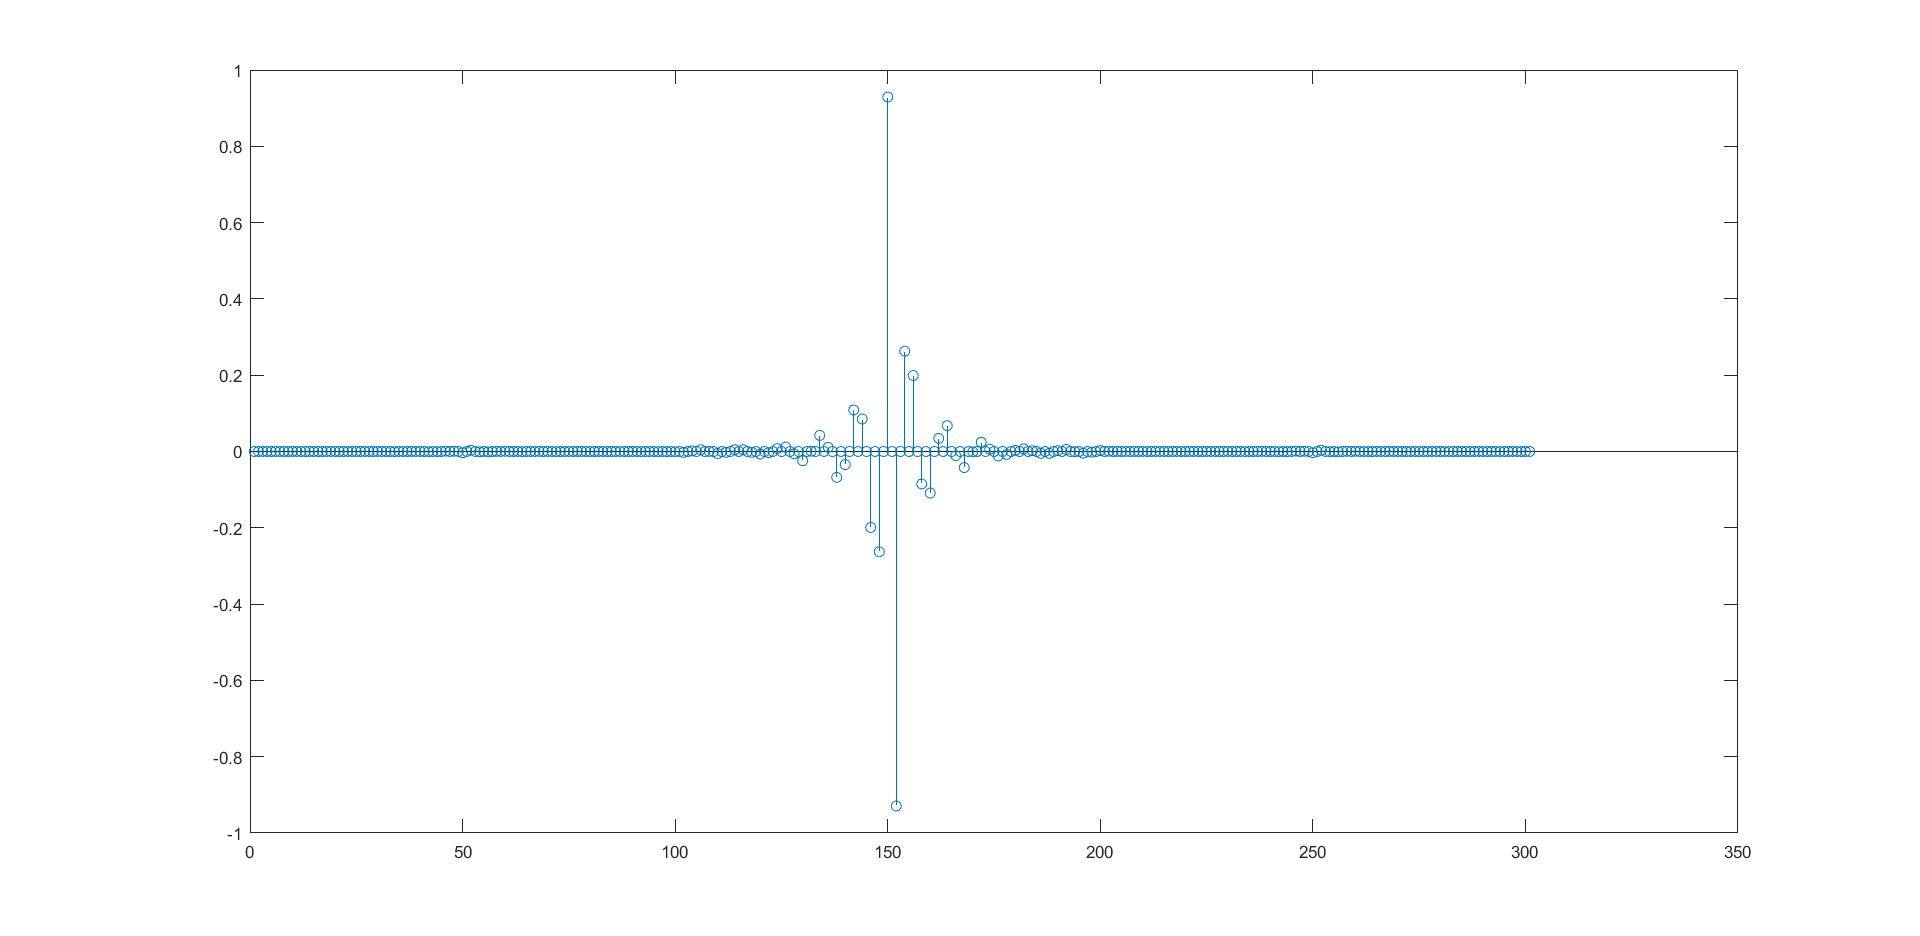
\includegraphics[width=1.3\textwidth]{4.jpg}%
\caption{Plot of $c_n$ unshifted : symmetric about $n$=150}%
\label{fig:proto}%
\end{figure}% 
 \\
\begin{figure}[th]%
\centering
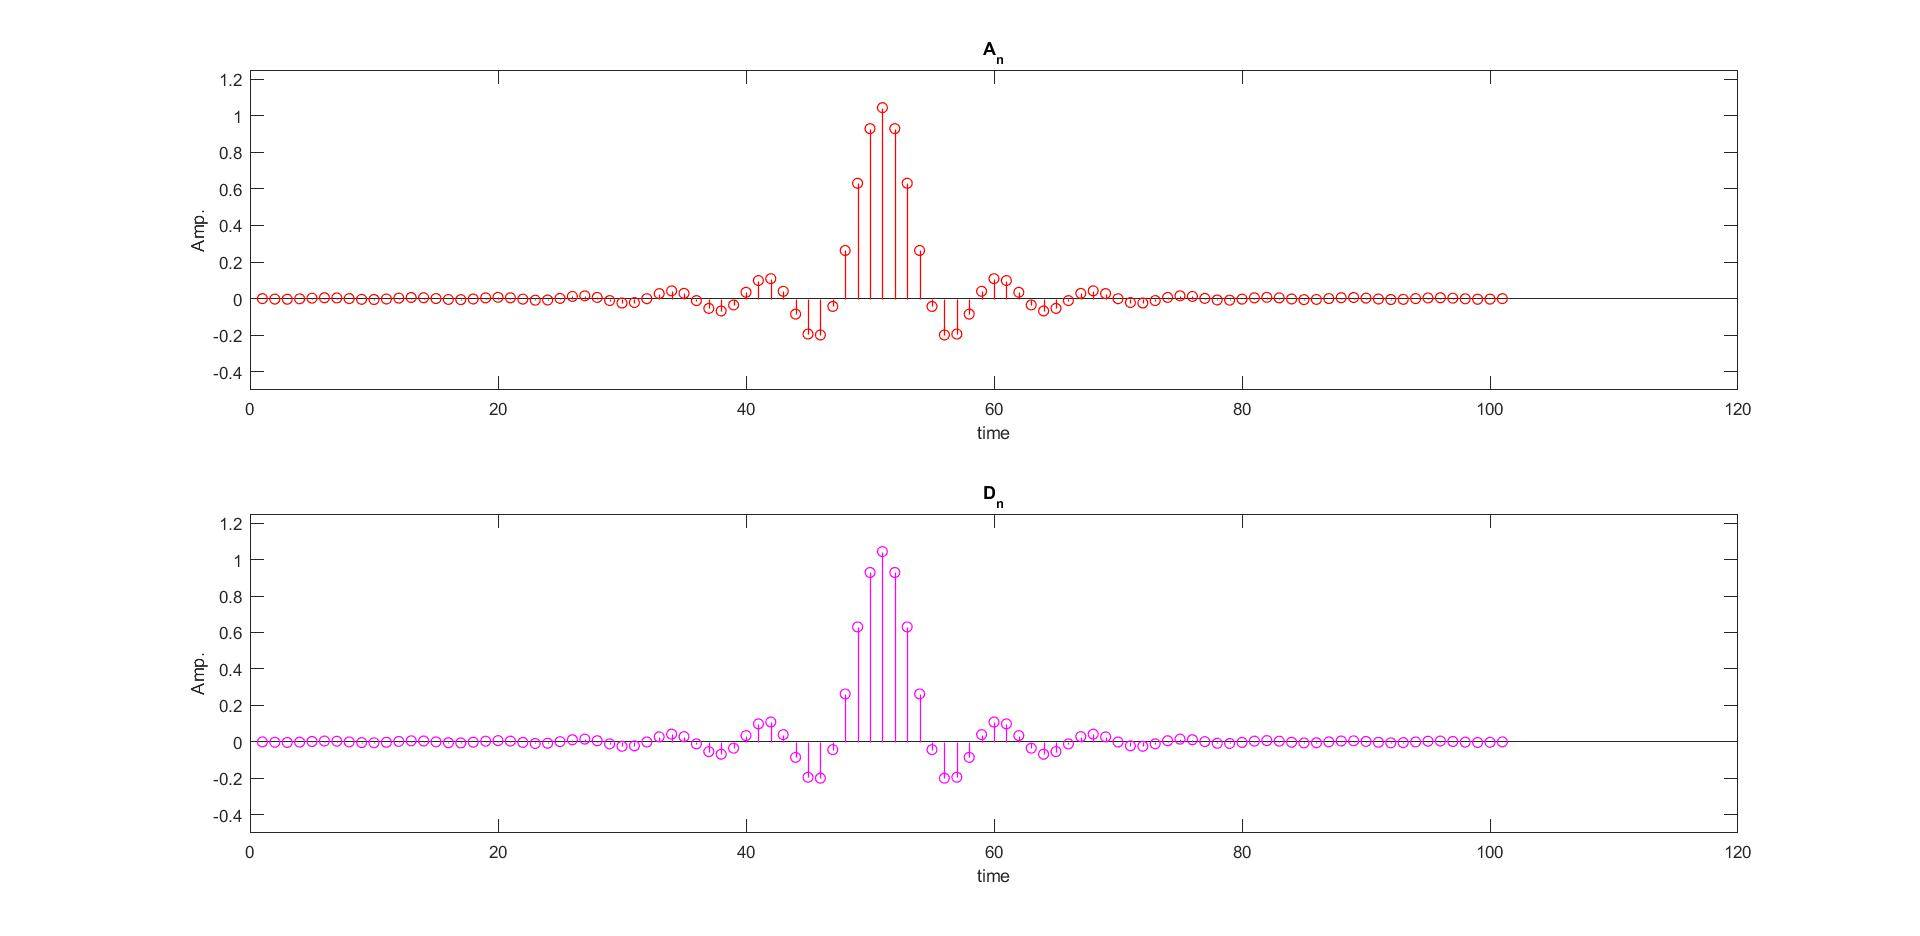
\includegraphics[width=1.3\textwidth]{3.jpg}%
\caption{(b).Plot of $A_n$ and $D_n$ vs time  in linear scale}%
\label{fig:proto}%
\end{figure}%

\begin{figure}[ht]%
\centering
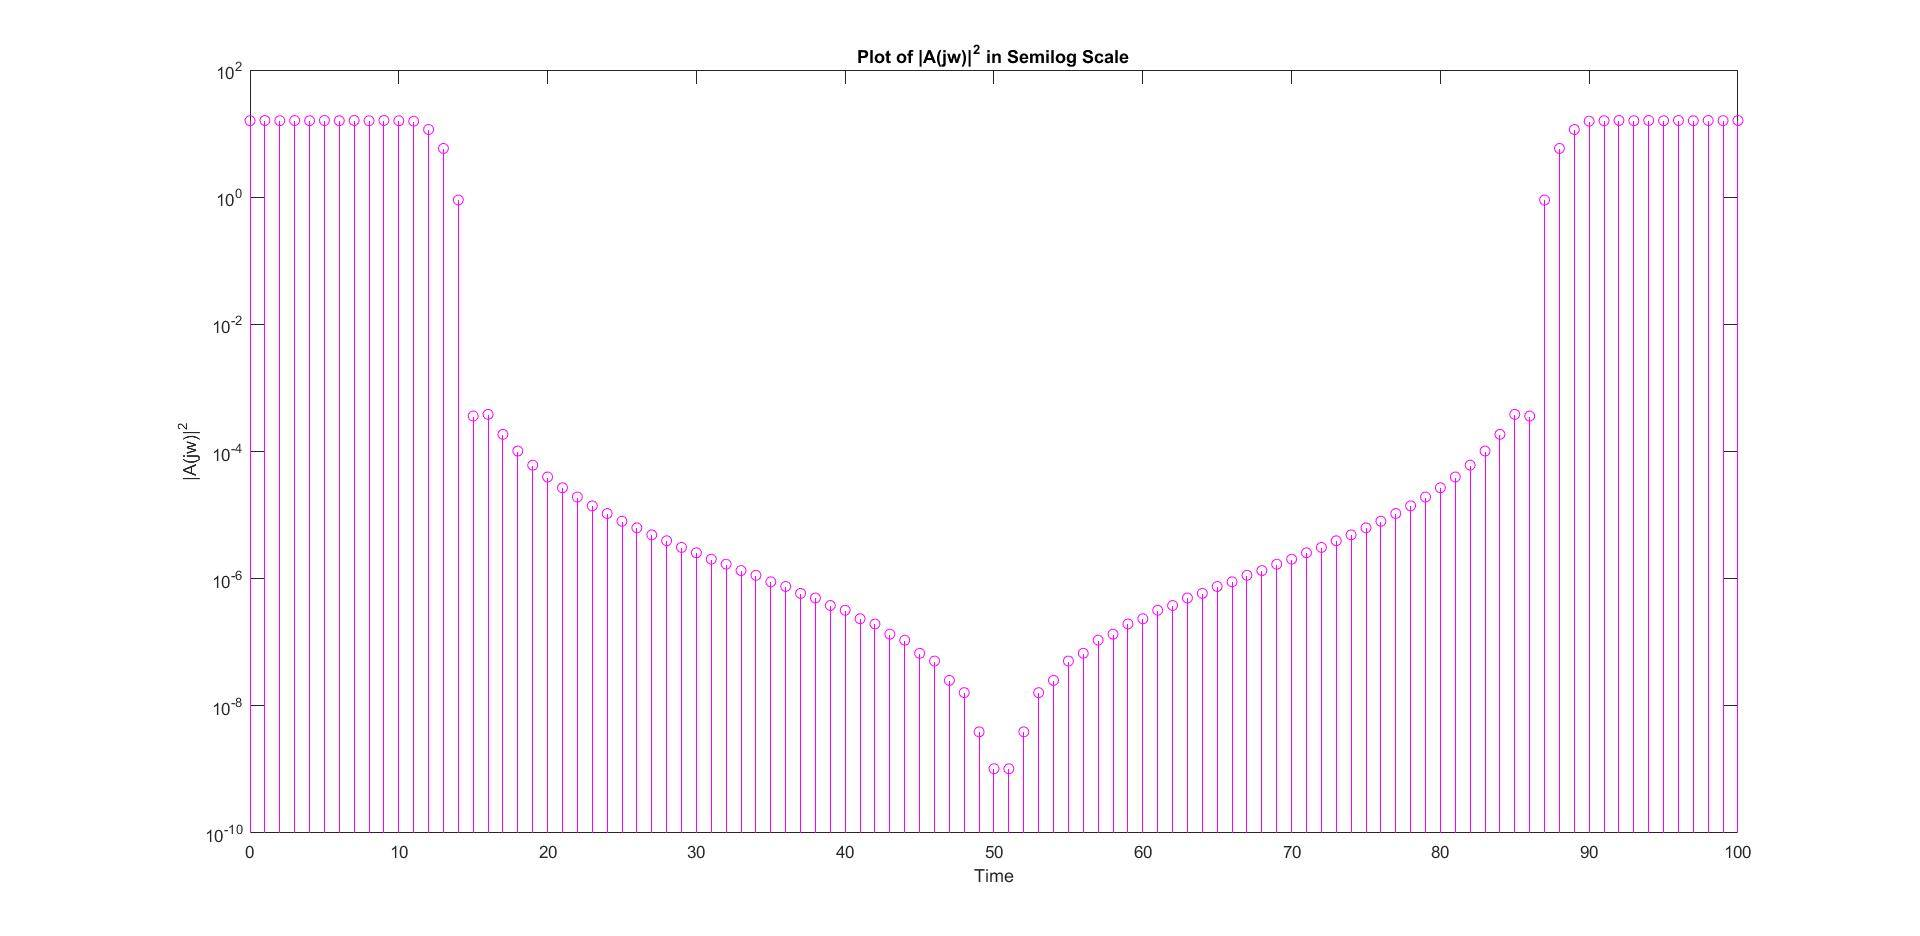
\includegraphics[width=1.3\textwidth]{1.jpg}%
\caption{(c).101-point DFT of $|A(w)|^2$ in semilog scale}%
\label{fig:proto}%
\end{figure}%
\begin{figure}[th]%
\centering
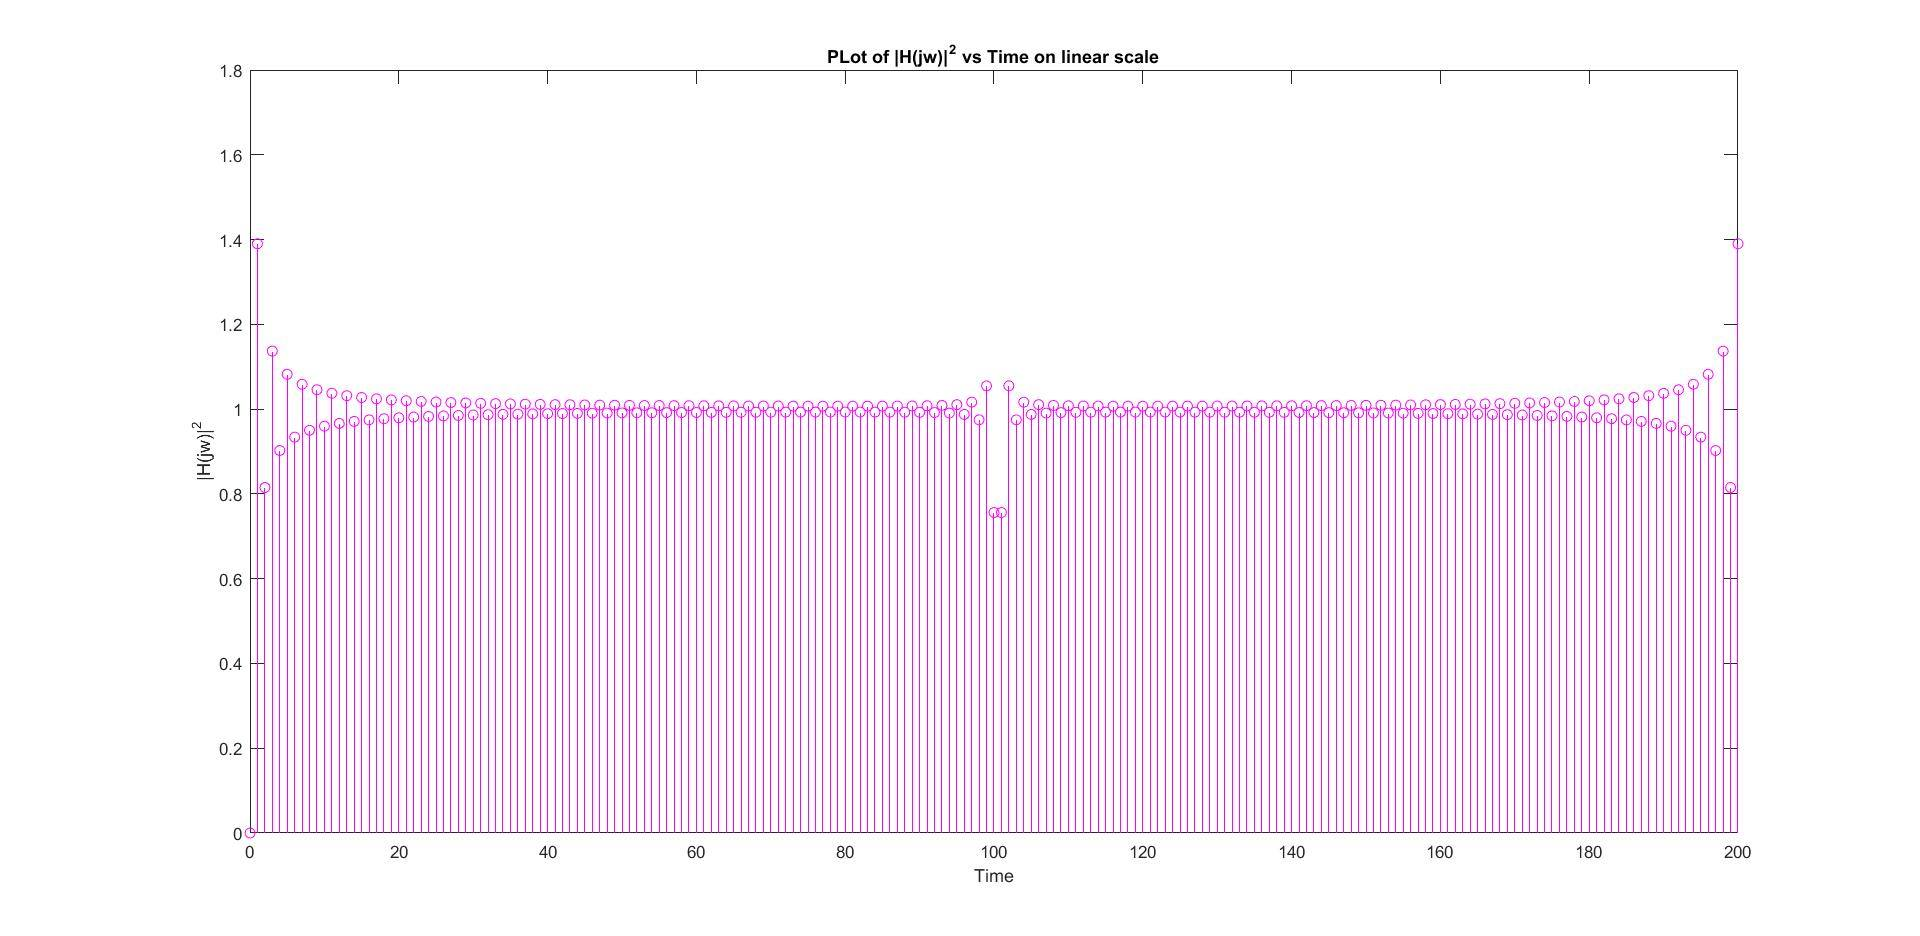
\includegraphics[width=1.3\textwidth]{2.jpg}%
\caption{(d).201-point DFT of $|H(w)|^2$ in linear scale}%
\label{fig:proto}%
\end{figure}%
\end{document}